\documentclass[a4paper, 12pt]{article}%тип документа

%%%Библиотеки
	%\usepackage[warn]{mathtext}	
	\usepackage[T2A]{fontenc} % кодировка
	\usepackage[utf8]{inputenc} % кодировка исходного текста
	\usepackage[english,russian]{babel} % локализация и переносы
	\usepackage{caption}
	\usepackage{listings}
	\usepackage{amsmath,amsfonts,amssymb,amsthm,mathtools}
	\usepackage{wasysym}
	\usepackage{graphicx}%Вставка картинок правильная
	\usepackage{float}%"Плавающие" картинки
	\usepackage{wrapfig}%Обтекание фигур (таблиц, картинок и прочего)
	\usepackage{fancyhdr} %загрузим пакет
	\usepackage{lscape}
	\usepackage{xcolor}
	\usepackage[normalem]{ulem}
	\usepackage{hyperref}

%%%Конец библиотек




%%%Настройка ссылок
	\hypersetup
	{
		colorlinks=true,
		linkcolor=blue,
		filecolor=magenta,
		urlcolor=blue
	}
%%%Конец настройки ссылок


%%%Настройка колонтитулы
	\pagestyle{fancy}
	\fancyhead{}
	\fancyhead[L]{Лабораторная работа}
	\fancyhead[R]{Талашкевич Даниил, группа Б01-009}
	\fancyfoot[C]{\thepage}
%%%конец настройки колонтитулы



							\begin{document}
						%%%%Начало документа%%%%


%%%Начало титульника
\begin{titlepage}

	\newpage
	\begin{center}
		\normalsize Московский физико-технический институт \\(госудраственный 			университет)
	\end{center}

	\vspace{6em}

	\begin{center}
		\Large Лабораторная работа по оптике\\
	\end{center}

	\vspace{1em}

	\begin{center}
		\large \textbf{Кольца Ньютона [4.2.1]}
	\end{center}

	\vspace{2em}

	\begin{center}
		\large Талашкевич Даниил Александрович\\
		Группа Б01-009
	\end{center}

	\vspace{\fill}

	\begin{center}
	Долгопрудный \\2022
	\end{center}
	
\end{titlepage}
%%%Конец Титульника



%%%Настройка оглавления и нумерации страниц
	\thispagestyle{empty}
	\newpage
	\tableofcontents
	\newpage
	\setcounter{page}{1}
%%%Настройка оглавления и нумерации страниц


					%%%%%%Начало работы с текстом%%%%%%

\section{Аннотация}

$\text{ }$

$\textbf{Цель работы}$ : ознакомление с явлением интерференции в тонких пленках (полосы равной толщины) на примере колец Ньютона и с методикой интерференционных измерений кривизны стеклянной поверхности.

$\textbf{В работе используются}$ : измерительный микроскоп с опак-иллюминатором; плосковыпуклая линза; пластинка из черного стекла; ртутная лампа ПРК-4; щель; линзы; призма прямого зрения; объектная пікала.

\section{Теоретические сведения}

Интерференция -- взаимное увеличение или уменьшение результирующей амплитуды двух или нескольких когерентных волн при их наложении друг на друга.

Кольца Ньютона -- кольцеобразные интерференционные максимумы и минимумы, появляющиеся вокруг точки касания слегка изогнутой выпуклой линзы и плоскопараллельной пластины при прохождении света сквозь линзу и пластину.

В нашей установке кольца Ньютона образуются при интерференции световых волн, отраженных от границ тонкой воздушной прослойки, заключенной между выпуклой поверхностью линзы и плоской стеклянной пластинкой (рис. 1). Наблюдение ведется в отраженном свете.

\begin{figure}[!h]
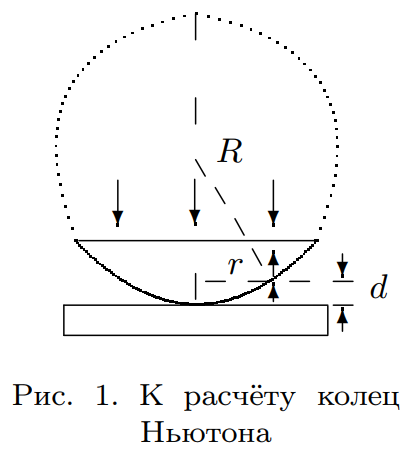
\includegraphics[scale=0.5]{1.png}
\caption{теоретическая модель}
\label{11}
\end{figure}

Этот классический опыт используется для определения радиуса кривизны сферических поверхностей линз. В этом опыте наблюдается интерференция волн, отражённых от границ тонкой воздушной прослойки, образованной сферической поверхностью линзы и плоской стеклянной пластиной. При нормальном падении света (рис. 1) интерференционные полосы локализованы на сферической поверхности и являются полосами равной толщины.
	
	Геометрическая разность хода между интерферирующими лучами равна удвоенной толщине воздушного зазора $ 2d $ в данном месте. Для точки на сферической поверхности, находящейся на расстоянии $ r $ от оси системы, имеем $ r^2 = R^2 - (R - d)^2 = 2Rd - d^2 $, где $ R $ -- радиус кривизны сферической поверхности (рис. \ref{11}).
	
	При $ R \gg d $ получим $d = r^2/2R $. С учётом изменения фазы на $ \pi $ при отражении волны от оптически более плотной среды (на границе воздух-стекло) получим \textbf{оптическую разность хода интерферирующих лучей}:
	
	\begin{equation}\label{r_m}
	\Delta = \dfrac{\lambda}{2} + 2d = \dfrac{r^2}{2R} + \dfrac{\lambda}{2}
	\end{equation}
	
	Из условия интерференционного минимума $ \Delta = \dfrac{(2m +1)\lambda}{2}, \; m =0, 1, 2, \dots $ . Получим радиусы темных колец $ r_m $, а из аналогичного условия максимума $ \Delta = m \lambda $ радиусы светлых $ r_m' $ :
	
	\begin{equation}\label{r_m'}
	r_m = \sqrt{m \lambda R}, \qquad 	r_m' = \sqrt{\dfrac{(2m-1)m \lambda R}{2}}
	\end{equation}


\section{Экспериментальная установка}

Схема экспериментальной установки приведена на рис. \ref{2}. Опыт выполняется с помощью измерительного микроскопа.
На столик микроскопа помещается держатель с полированной пластинкой из
чёрного стекла. На пластинке лежит исследуемая линза.

	\begin{figure}[!h]
	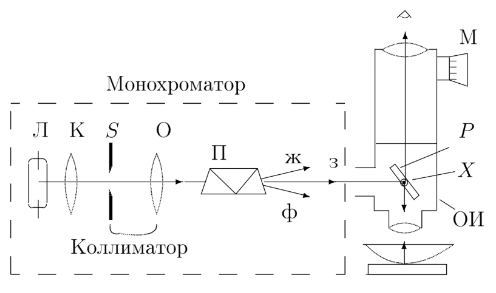
\includegraphics[width=\linewidth]{2.png}
	\caption{Экспериментальная установка}
	\label{2}
	\end{figure}

	Источником света служит ртутная лампа, находящаяся в защитном кожухе. Для получения монохроматического света применяется призменный монохроматор, состоящий из конденсора $ К $, коллиматора (щель $ S $ и объектив $ О $) и призмы прямого зрения $ П $. Эти устройства с помощью рейтеров располагаются на оптической скамье. Свет от монохроматора попадает на расположенный между объективом и окуляром микроскопа опак-иллюминатор (ОИ)  специальное устройство, служащее для освещения объекта при работе в отражённом свете. Внутри опак-иллюминатора находится полупрозрачная стеклянная пластинка P, наклоненная под углом $ 45^\circ $ к оптической оси микроскопа. Свет частично отражается от этой пластинки, проходит через объектив микроскопа и попадает на исследуемый объект. Пластинка может поворачиваться вокруг горизонтальной оси $ X $, опак-иллюминатор вокруг вертикальной оси.

	Столик микроскопа может перемещаться в двух взаимно перпендикулярных направлениях помощью винтов препаратоводителя. Отсчетный крест окулярной шкалы перемещается перпендикулярно оптической оси с помощью микрометрического винта $ М $.
	
	Оптическая схема монохроматора позволяет получить в плоскости входного окна опак-иллюминатора достаточно хорошо разделённые линии спектра ртутной лампы. Изображение щели $ S $ фокусируется на поверхность линзы объективом микроскопа, т.е. точка источника и точка наблюдения спектра совпадают.Интерференционная картина не зависит от показателя преломления линзы и определяется величиной зазора между линзой и пластинкой (кольца равной толщины).

	Сначала микроскоп настраивается на кольца Ньютона в белом свете (свете ртутной лампы), затем при помощи монохроматора выделить из спектра яркую зелёную линию и провести измерения диаметров колец в монохроматическом свете. 
	

\section{Ход работы}

Сперва настроим микроскоп для наблюдения картины колец Ньютона. Аналогично для получения последних необходимо настроить монохроматор. Измерения будем проводить в безразмерных единицах окулярной шкалы, а для получения реальных величик впоследствии будем использовать калиброванную объектную шкалу.

\subsection{Радиусы колец Ньютона и кривизна линзы}

Для определения радиуса кривизны линзы будем измерять диаметры колец, результаты измерений занесем в таблицу \ref{tab1}. По этим данным, зная длину волны $\lambda$, рассчитаем радиус $R$ кривизны линзы.

\subsection{Наблюдение «биений»}

При биениях мы наблюдали следующее количество полос между центрами четких систем $\Delta m=18 .$ Вычислим отсюда разность длин волн желтого и зеленого света ртутной лампы $\Delta \lambda=\lambda_{\text {ж }}-\lambda_{\text {з }}$ :
$$
(\Delta m+1) \lambda_{3}=\Delta m \lambda_{\text {ж }} \Rightarrow \Delta \lambda=\frac{\lambda_{3}}{\Delta m} \approx 30 \text { нм }
$$

Теоретические данные:

\[ \text{Длина волны желтого и зеленого света: } \lambda_{\text {ж }} = 583 \text{ нм}, \lambda_{\text {з }} = 550 \text{ нм} \Rightarrow \]

\[ \Rightarrow \Delta \lambda_{\text{теор}} = 33 \text{ нм}.\]

Относительное отклонение экспериментального значения от теоретического:

\[ \varepsilon_{\Delta \lambda} = \frac{|30 - 33|}{33} \approx 9\% \]

\subsection{Калибровка окулярной шкалы}

Для определения цены деления окулярной шкалы сверху на линзу кладем калиброванную объектную шкалу.
Объектная шкала размером 1 мм разбита на 100 делений. Используя всё поле зрения микроскопа, отмечаем, какие из самых дальних штрихов объектной шкалы лучше всего совпадают со штрихами окулярной шкалы.

Отнормировав шкалу с калибровочной объектной шкалы, найдем:
$$
\delta x=\frac{0.79_{\mathrm{MM}}}{8}=0.099 \pm 0.001 \text{ мм}
$$

\section{Обработка данных}

\subsection{Белые и темные кольца}

\begin{table}[h!]
		\begin{center}
			\begin{tabular}{|c|c|c|c|c|c|c|}
				\hline
				m & \multicolumn{3}{|c|}{Темные кольца} & \multicolumn{3}{|c|}{Светлые кольца} \\
				\cline{2-7}
				& $ l_1 $& $ l_2 $ & $ r_{m\text{,темн}}^2 $ &$ l_1 $& $ l_2 $ & $ r_{m\text{, светл}}^2 $ \\
				\hline
				0 & 4,71 & 3,72 & 0,25 & 4,15 & 4,15 & 0,00 \\
				1 & 5,00 & 3,24 & 0,77 & 4,78 & 3,43 & 0,46 \\
				2 & 5,45 & 2,92 & 1,60 & 5,16 & 3,08 & 1,08 \\
				3 & 5,59 & 2,65 & 2,16 & 5,44 & 2,79 & 1,76 \\
				4 & 5,83 & 2,42 & 2,91 & 5,70 & 2,54 & 2,50 \\
				5 & 6,02 & 2,23 & 3,59 & 5,91 & 2,32 & 3,22 \\
				6 & 6,17 & 2,06 & 4,22 & 6,09 & 2,11 & 3,96 \\
				7 & 6,47 & 1,89 & 5,24 & 6,25 & 1,97 & 4,58 \\
				\hline
			\end{tabular}
		\end{center}
		\caption{данные для измерение диаметров колец Ньютона}
		\label{tab1}
	\end{table}

Построим график зависимости $r_m^2 (m)$, откуда сможем найдем радиус кривизны линзы:

\newpage

	\begin{figure}[!h]
	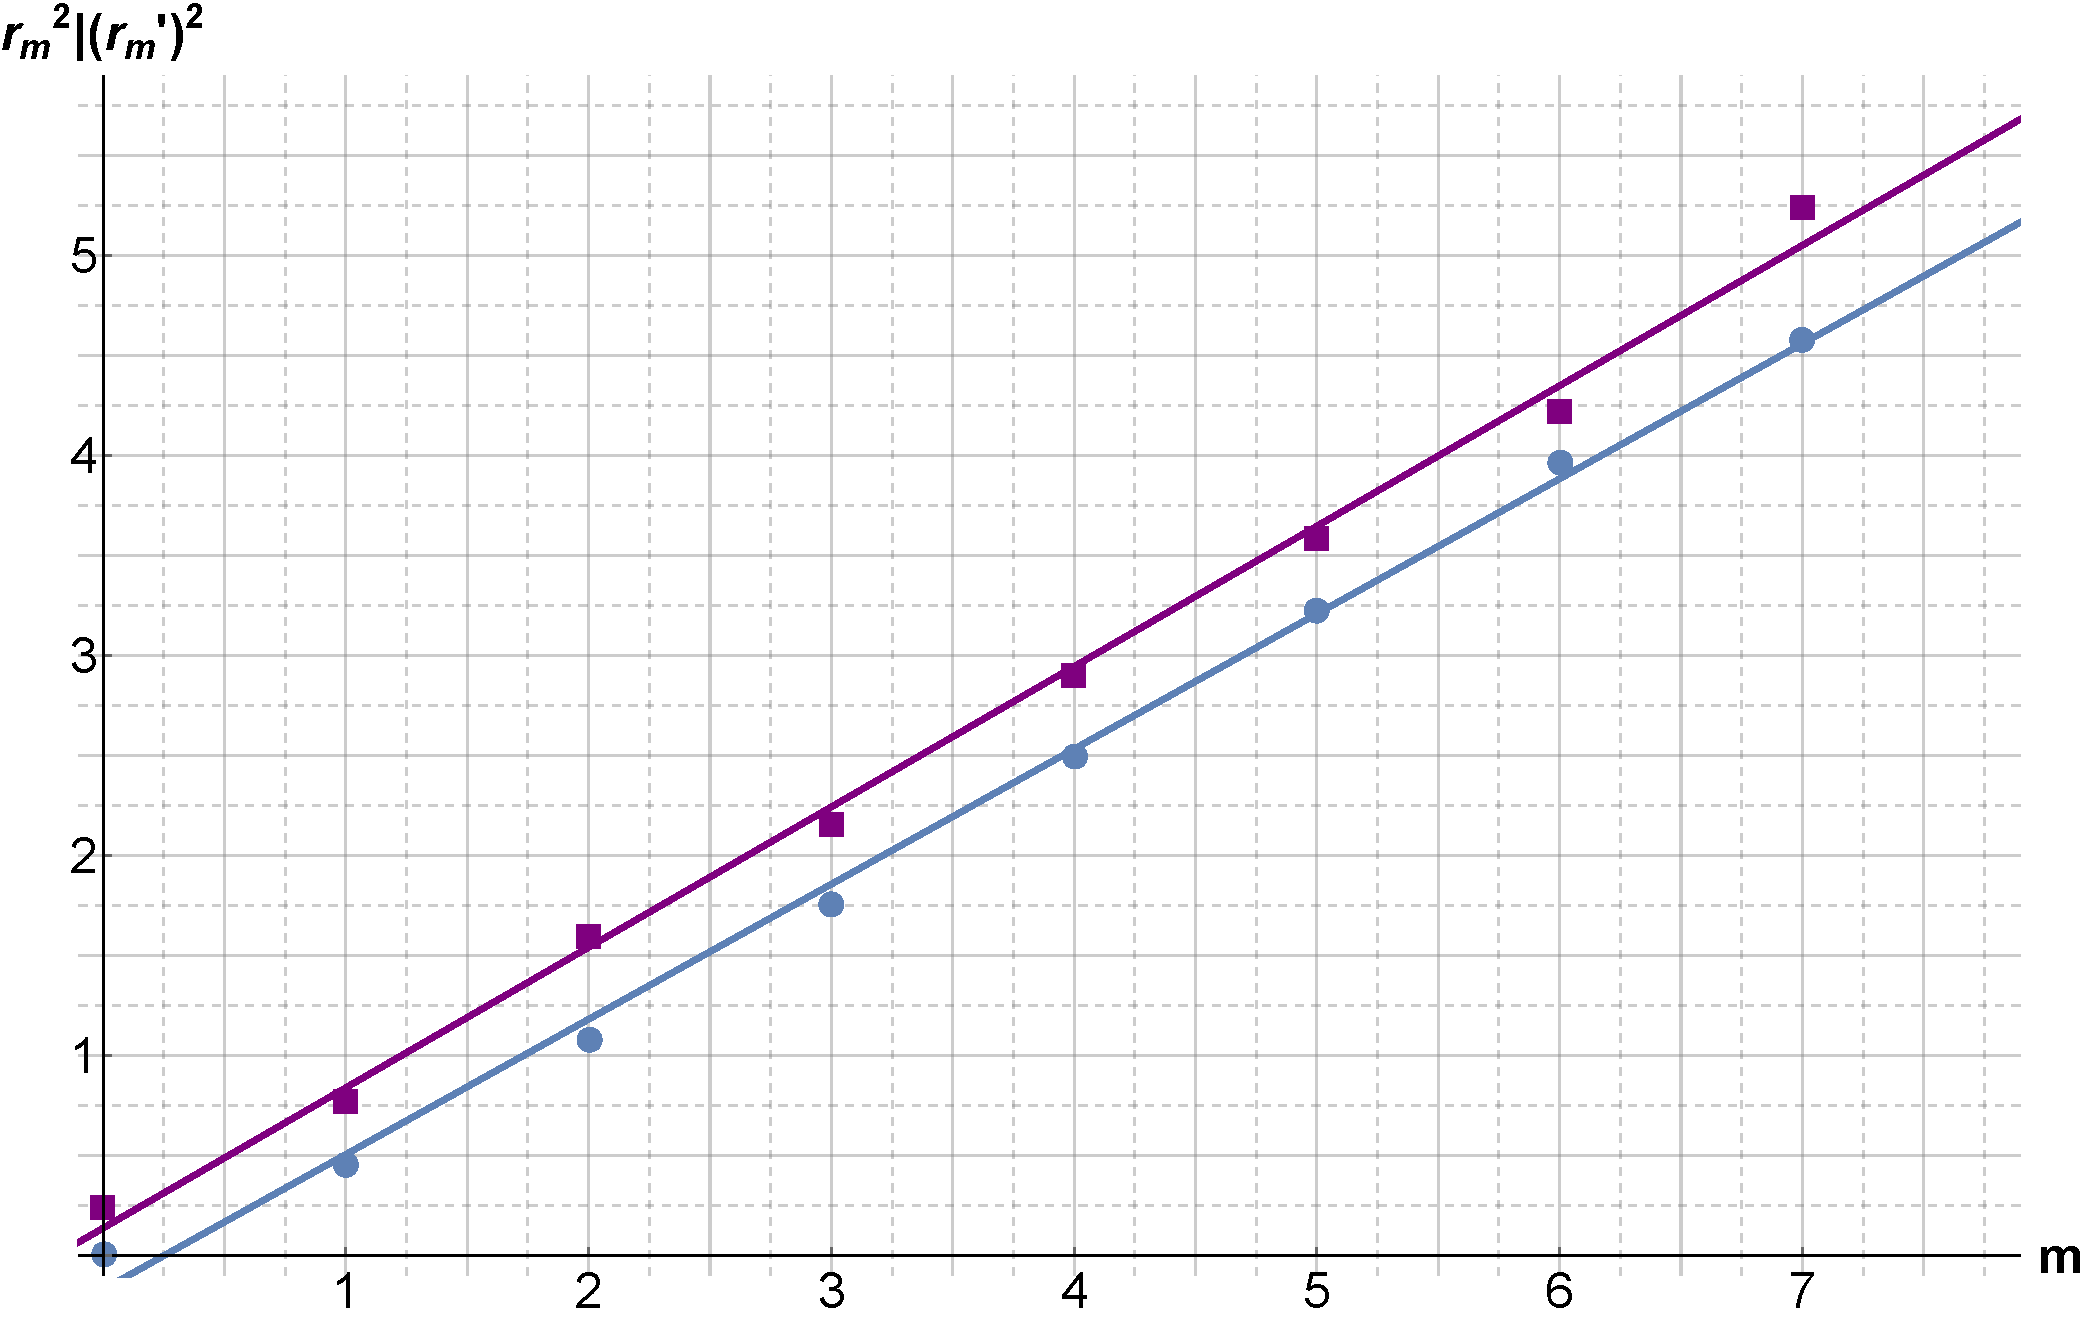
\includegraphics[width=\linewidth]{graph1.pdf}
	\caption{график зависимости $r_m^2 (m)$}
	\label{2}
	\end{figure}

Найдем коэффициент пропорциональности по МНК, также оценим погрешность:

Вычислим коэффициенты $a$ и $b$ уравнения линейной регрессии $\hat{y}=a x+b$ по известным формулам:

$$
\begin{aligned}
&a=\frac{\sum x_{i} \sum y_{i}-n \sum x_{i} y_{i}}{\left(\sum x_{i}\right)^{2}-n \sum x_{i}^{2}}=\frac{28 \cdot 20,74-8 \cdot 102,04}{28^{2} - 8 \cdot 140} \approx 0,70 ; \\
&b=\frac{\sum x_{i} \sum x_{i} y_{i}-\sum x_{i}^{2} \sum y_{i}}{\left(\sum x_{i}\right)^{2}-n \sum x_{i}^{2}}=\frac{28 \cdot 102,04-140 \cdot 20,74}{28^{2} - 8 \cdot 140} \approx 0,14 .
\end{aligned}
$$

Вычислим коэффициенты линейной парной корреляции $\left(r_{x y}\right)$ и детерминации $\left(R^{2}\right):$
$$
r_{x y}=\frac{n \sum x_{i} y_{i}-\sum x_{i} \sum y_{i}}{\sqrt{\left(n \sum x_{i}^{2}-\left(\sum x_{i}\right)^{2}\right)\left(n \sum y_{i}^{2}-\left(\sum y_{i}\right)^{2}\right)}}=\frac{8 \cdot 102,04-28 \cdot 20,74}{\sqrt{\left(8 \cdot 140-28^{2}\right)\left(8 \cdot 74,5032-20,74^{2}\right)}};
$$

$$ r_{xy} \approx 0,998 $$
следовательно, $R^{2}=r_{x y}^{2}=0,998^{2} \approx 0,9959 .$

Для оценки значимости параметров регрессии и корреляции сначала:
$$
\begin{aligned}
&\text { - найдём } x \text { средний: } \bar{x}=\frac{1}{n} \sum x_{i}=\frac{28}{8}=3.5 ; \\
&\text { - составим таблицу вспомогательных величин, где } \varepsilon_{i}=y_{i}-\hat{y}_{i}, \\
&\Delta \varepsilon_{i}=\varepsilon_{i}-\varepsilon_{i-1}, A_{i}=\left|\frac{y_{i}-\hat{y}_{i}}{y_{i}}\right|:
\end{aligned}
$$

\begin{tabular}{|c|c|c||c|c|c|c|c|c|c|c|}
\hline$i$ & $x_{i}$ & $y_{i}$ & $\hat{y}_{i}$ & $x_{i}-\bar{x}$ & $\left(x_{i}-\bar{x}\right)^{2}$ & $\varepsilon_{i}$ & $\varepsilon_{i}^{2}$ & $A_{i}$ & $\Delta \varepsilon_{i}$ & $\left(\Delta \varepsilon_{i}\right)^{2}$ \\
\hline 1 & 0 & $0,25$ & $0,14$ & $-3,5$ & $12,25$ & $0,11$ & $0,013$ & $0,447$ & $-$ & $-$ \\
\hline 2 & 1 & $0,77$ & $0,84$ & $-2,5$ & $6,25$ & $-0,07$ & $0,005$ & $0,090$ & $-0,181$ & $0,032$ \\
\hline 3 & 2 & $1,6$ & $1,54$ & $-1,5$ & $2,25$ & $0,06$ & $0,004$ & $0,037$ & $0,129$ & $0,017$ \\
\hline 4 & 3 & $2,16$ & $2,24$ & $-0,5$ & $0,25$ & $-0,08$ & $0,007$ & $0,038$ & $-0,141$ & $0,020$ \\
\hline 5 & 4 & $2,91$ & $2,94$ & $0,5$ & $0,25$ & $-0,03$ & $0,001$ & $0,011$ & $0,049$ & $0,002$ \\
\hline 6 & 5 & $3,59$ & $3,64$ & $1,5$ & $2,25$ & $-0,05$ & $0,003$ & $0,015$ & $-0,021$ & $0,001$ \\
\hline 7 & 6 & $4,22$ & $4,35$ & $2,5$ & $6,25$ & $-0,13$ & $0,016$ & $0,030$ & $-0,071$ & $0,005$ \\
\hline 8 & 7 & $5,24$ & $5,05$ & $3,5$ & $12,25$ & $0,19$ & $0,037$ & $0,037$ & $0,319$ & $0,102$ \\
\hline$\sum$ & $-$ & $-$ & $-$ & $-$ & 42 & $-$ & $0,08$ & $0,705$ & $-$ & $0,179$ \\
\hline
\end{tabular}


Случайные ошибки параметров $a, b$ и коэффициента корреляции $r_{x y}$:

$$
\begin{aligned}
&m_{a}=\sqrt{\frac{1}{\sum\left(x_{i}-\bar{x}_{i}\right)^{2}} \cdot \frac{\sum\left(y_{i}-\hat{y}_{i}\right)^{2}}{n-2}}=\sqrt{\frac{1}{42} \cdot \frac{0.0847}{8-2}} \approx 0,0183 ; \\
&m_{b}=\sqrt{\frac{\sum\left(y_{i}-\hat{y}_{i}\right)^{2}}{n-2} \cdot \frac{\sum x_{i}^{2}}{n \sum\left(x_{i}-\bar{x}_{i}\right)^{2}}}=\sqrt{\frac{0.0847}{8-2} \cdot \frac{140}{8 \cdot 42}} \approx 0,0767 ;
\end{aligned}
$$
	
Полученные значения:

\[ a_{\text{с}} = 0,70 \pm 0,02  \]
\[ b_{\text{с}} = 0,14 \pm 0,08  \]

Аналогичные рассчеты для светлых колец дают:

\[ a_{\text{т}} = 0,68 \pm 0,02  \]
\[ b_{\text{т}} = -0,17 \pm 0,06 \]

\subsection{Радиус линзы}

Из теории и по полученным данным (зависимости $r_m^2 (m)$) найдем радиус кривизны линзы:

\[ R=\frac{r_{m}^{2}}{m \lambda} = \frac{a_{\text{т}}}{\lambda} = (1,26 \pm 0,04) \text{ см} .\]


\section{Вывод}

В ходе выполнения данной работы экспериментально мы смогли пронаблюдать за картиной интерференционных максимумов и минимумов (кольца Ньютона), был рассчитан радиус кривизны линзы при помощи построения графики зависимости радиусов колец (темных и светлых) от их порядковых номеров. Полученные результаты:

\[ R = (1,26 \pm 0,04) \text{ см} .\]

Также мы рассчитали разницу длин волн желтого и зеленого света ртутной лампы: 

\[ \Delta \lambda_{\text{эксп}} = 30, \Delta \lambda_{\text{теор}} = 33 \text{ нм}\]

\[ \varepsilon_{\Delta \lambda} = \frac{|30 - 33|}{33} \approx 9\% \]

Разница в результатах объясняется погрешностью определения $m$.

\section{Литература}

\begin{enumerate}

\item Лабораторный практикум по общей физике. В 3 т. Том 2. Оптика: учебное пособие

\item http://mathhelpplanet.com (МНК и регрессионный анализ)

\item https://ru.wikipedia.org/wiki/Свет (длины волн желтого и зеленого света)

\end{enumerate}	

\end{document}
